%% Intended to be included into a larger document
\chapter{Related Work}

This chapter lays out previously conducted work that relates to my research area. As this topic is an area of rapid innovation, some of the references exist only as web pages, not as works in peer-reviewed publications. 

\section{Climate Change}
\label{sec:climate-change}

In 2007, the Intergovernmental Panel on Climate Change released its fourth assessment report \cite{IPCC-synthesis-report-2007}. The conclusions of this long-running analysis of studies on climate change and its effects are widely accepted as the consensus of the world's scientific community. They found that there is broad agreement that the climate is warming: air and ocean temperatures are higher, snow and ice are melting, and sea levels are rising. Further, natural systems are being affected: plant and animal ranges are moving upward, and there are changes in fish and algae due to rising ocean temperatures.

The IPCC found that the warming of the climate was very likely due to anthropogenic greenhouse gas (GHG) emissions. GHG emissions from humans have increased by 70\% between 1970 and 2004. While there are a variety of GHG that impact climate change, \COtwo is the most important of the human-caused GHGs. Sea level rise in the second half of the 20th century was also very likely caused by humans, and rising sea levels have a potentially enormous impact on island communities like Hawai`i.

With current climate change policies, GHG emissions are projected to continue to increase this century. Further, there is no single technology that will mitigate the problem of climate change; a range of policies and innovations is required. The report lists both energy efficiency and individual behavior modification as suggested GHG mitigation strategies.

\subsection{Focus on Carbon}

When discussing gasses in the atmosphere that are linked to climate change, there are a several terms. Greenhouse gas (GHG) is the most general term, referring to any gas in the atmosphere that leads to a greenhouse effect, trapping thermal radiation from the sun in the Earth's atmosphere. There are several GHGs in Earth's atmosphere: water vapor (H$_2$O), carbon dioxide (\COtwo), methane (CH$_4$), nitrous oxide (N$_2$O), ozone (O$_3$), and others. Each gas has different greenhouse effects on a molecule-by-molecule basis; for example, methane has a much greater greenhouse effect than carbon dioxide.  However, carbon dioxide (henceforth referred to as \COtwo) is found in much greater quantities in the atmosphere than methane. Water vapor is the largest component of the greenhouse effect, but it's contribution is not growing rapidly as \COtwo is and humans don't have as much control over water vapor as they do over \COtwo emissions.

For these reasons, most climate change mitigation focuses on \COtwo emissions. In this context, sometimes \COtwo is referred to as simply carbon, as in \emph{carbon footprint}. For my purposes here, the terms GHG, \COtwo, and carbon can largely be considered interchangeable except when distinctions between \COtwo and other GHGs are being discussed.

\subsection{Does Energy Efficiency Reduce Carbon Emissions?}

Many governmental plans to reduce GHG emissions involve improving energy efficiency in the home, in industry, and in transportation. While intuitively it would seem that increased energy efficiency would lead to decreased energy usage and thereby reduced GHG emissions, surprisingly there is some evidence both theoretical and empirical that energy efficiency actually increases energy usage! Saunders dubbed this unintuitive notion the Khazzoom-Brookes Postulate based on conclusions reached independently by those two researchers \cite{saunders-1992}. \fxnote{Insert references to Khazzoom and Lovins papers here, after I read them.}

Using neoclassical growth theory, Saunders finds that increased energy efficiency makes energy seem cheaper, thus allowing it to be substituted for labor in production. Increased energy efficiency also increases overall economic growth, which leads to increased overall energy usage.

In discussing this effect, rebound is defined as the difference between the expected amount of energy savings from an improvement in energy efficiency, and the actual observed effect. For example, if an improvement in metal smelting technology reduces the energy required to smelt by 20\%, but the energy consumed by the metal smelting industry only goes down by 10\% then the rebound is 50\%. If the rebound is greater than 100\%, then backfire is taking place (the efficiency measure has backfired) \cite{Hanley2008Do-increases-in}. There is some debate over whether the predicted increases will actually take place in the real world. Laitner suggests via a simple analysis that the rebound effect is small (2.4\%) \cite{Skip-Laitner:2000yg}. His equation relates future carbon emissions to current carbon emissions, increases in GDP and energy costs, and elasticities of income and energy prices to arrive at this conclusion. He goes on to a further analysis done by the Environmental Protection Agency and Lawrence Berkeley National Labs using the National Energy Modeling System showing that an ``energy-efficient/low-carbon technology path'' would suffer from a rebound effect of only 2.2\%. However, he acknowledges that consumer choices about energy usage could erode gains from efficiency, such as turning up the furnace thermostat because the cost of doing so has been effectively reduced.

The issue of consumer choices is a real one. Over the last 25 years, automobiles have been made more efficient through ``increasing the efficiency of the engine and transmission, decreasing weight, improving tires and reducing drag'' \cite{Heywood2008Fueling-Our-Future}. However, these improvements have been traded for vehicles that are larger, heavier, and faster, which has led to only modest improvements in overall fuel efficiency. This is an example of how energy efficiency may not always lead to reduced GHG emissions without motivating automobile users (and manufacturers) to buy and make fuel efficient vehicles.

Other authors find that rebound and even backfire are the likely results of economy-wide improvements in energy efficiency. The analysis of Hanley et al finds that backfire occurs when economy-wide improvements in energy efficiency are made \cite{Hanley2008Do-increases-in}. Their theoretical analysis finds that if energy demand is relatively price-elastic (demand increases when prices are low and reduces when prices are high), then backfire will occur. Empirical evidence of rebound and backfire are hard to come by because there are indirect system-wide effects due to the increased efficiency, and these indirect effects are difficult to measure. The authors created a Computable General Equilibrium (CGE) model of Scotland that simulates the economy and environmental impacts based on the inputs and outputs of the system. Using this model, almost all scenarios eventually end up in backfire. They note that since non-renewable energy sources use more energy in their production than renewable sources, increased energy efficiency actually reduces the percentage contribution of energy from renewable sources. They also urge caution when reviewing sustainability measures such as the ratio of Gross Domestic Product (GDP) to energy usage or carbon emissions, because even if the ratio increases (less carbon per unit GDP), if the GDP as a whole increases faster then the absolute carbon emitted will increase. They suggest that backfire could be prevented by combining energy efficiency improvements with taxes on energy use or a carbon tax. Since energy efficiency effectively reduces the cost of energy, the savings could offset the cost of additional taxes, thereby blunting any impact on economic activity.

It would appear that any energy efficiency improvements will have some degree of rebound effect, thus a naive pursuit of energy efficiency without taking into account the context around the improvements could risk reducing their effectiveness or even making them counterproductive! While many of the analyses deal at the macroeconomic level, it is not hard to think of individual scenarios where efficiency could actually increase personal usage, such buying two energy efficient refrigerators to replace one older energy-hogging refrigerator. Fortunately, the research plan I am pursuing is quite different: users learn about their GHG emissions (including energy usage) and based on that they decide on what actions to take, which could include increasing energy efficiency. The key to ensuring that energy efficiency improvements on the micro level lead to less GHG emissions is to combine efficiencies with changes in behavior. With the public's increased awareness of climate change, this should be a viable proposition.

\section{Energy Feedback}

One of the many ways that global GHG emissions can be reduced is through encouraging individuals to use less energy. To reduce energy use one must know how much energy one is using. Feedback systems display the consumption of a resource (such as electricity) to the user, usually in real time. Darby provides a detailed survey of studies on electricity feedback systems from the past 3 decades \cite{darby-review-2006}. The survey of 20 studies finds that, on average, the introduction of a direct (real-time) feedback system leads to reductions of energy usage ranging from 5-15\%. Feedback systems providing historical data (such as those provided with billing statements) are not as effective (0-10\% savings), but can be useful for assessing the impact of efficiency measures such as improved insulation or a more energy efficient appliance, since those savings accumulate over time.

Darby found that ``consumption in identical homes, even those designed to be low-energy dwellings, can easily differ by a factor of two or more depending on the behaviour of the inhabitants.'' This demonstrates the significant potential to curb energy usage (and thereby GHG emissions) through changes in individual's behavior.

\begin{figure}[htbp]
	\begin{center}
		\includegraphics[scale=0.59]{current-energy-website}
		\caption{View of LBNL's Current Energy Web Site on December 15, 2004}
		\label{fig:current-energy-website}
 	\end{center}
\end{figure}

During California's energy crisis in 2000 and 2001, Lawrence Berkeley National Laboratory created a web site that graphed data from utilities \cite{Bartholomew2008Current-Energy}. The graphs showed consumer demand for electricity (actual and forecast), and the utilities' generation capacity (see \autoref{fig:current-energy-website} for an example graph). Darby reports anecdotal evidence that people viewing the graphs changed their electricity usage based on the data \cite{darby-review-2006}.

There is also evidence that just the knowledge that one is being monitored can cause one to consume fewer resources. A group of researchers simulating a mission to Mars or the Moon in the Canadian Arctic for four months tracked the crew member's water usage \cite{Bamsey2008FMARS}. Water usage was monitored via automated meters during the entire mission, but during certain multi-day study periods, crew members were also required to manually log their water usage at the point of use. The authors found that water usage was 10\% less during these study periods. The reduced water usage could be due to the knowledge that the usage was being examined more closely, or perhaps the extra effort required to manually record their water usage led to crew members reducing non-essential water use (see \autoref{ecoisland} for another possible benefit to manual data collection).

While feedback can increase energy conservation, there are still cultural norms that strongly influence what behaviors are non-negotiable. Strengers performed an ethnographic study of 10 households participating in a smart metering trial to examine how their comfort and cleanliness norms affected their energy savings \cite{strengers-comfort-norms-2008}. Participants were provided with metering devices that displayed electricity and water usage, and greenhouse gas emissions in real time. The author was attempting to use feedback to change the participants societal norms for comfort and cleanliness. For example, until relatively recently, bathing weekly was the norm, but now bathing daily is considered normal behavior. Like many people, the participants did not understand connection between the consumption data and their practices. Participants tended to increase conservation by changing technology (such as using CFLs instead of incandescent light bulbs), or by minor behavioral changes like ``taking shorter showers, doing full loads of laundry''.

Strengers states that people act the way they do (in matters of cleanliness and comfort) because ``they believe society expects them to'' and because many companies and organizations have a vested interest in keeping it that way. Therefore just providing people information about their consumption is not enough, because individuals are constrained by infrastructures and social norms. She suggests increasing social interaction regarding the feedback system by making placement more prominent and encouraging discussion with household visitors, since people try to conform to the expectations of their peers.
However, it would seem that changing societal norms is one of the hardest possible means for reducing consumption. It also feeds into many of the negative stereotypes of environmentalism: stinky people living in dark, cold homes. Despite the irrationality of some of these norms, effort may be better spent focusing on areas where the effort will meet less resistance.

\begin{figure}[htbp]
	\begin{center}
		\subfigure[Device itself]{\label{fig:thighmaster-device}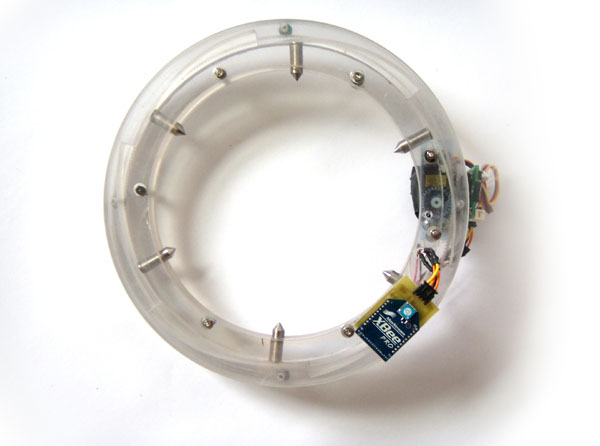
\includegraphics[height=2.5in]{thighmaster-alone}}
		\subfigure[As worn on leg]{\label{fig:thighmaster-leg}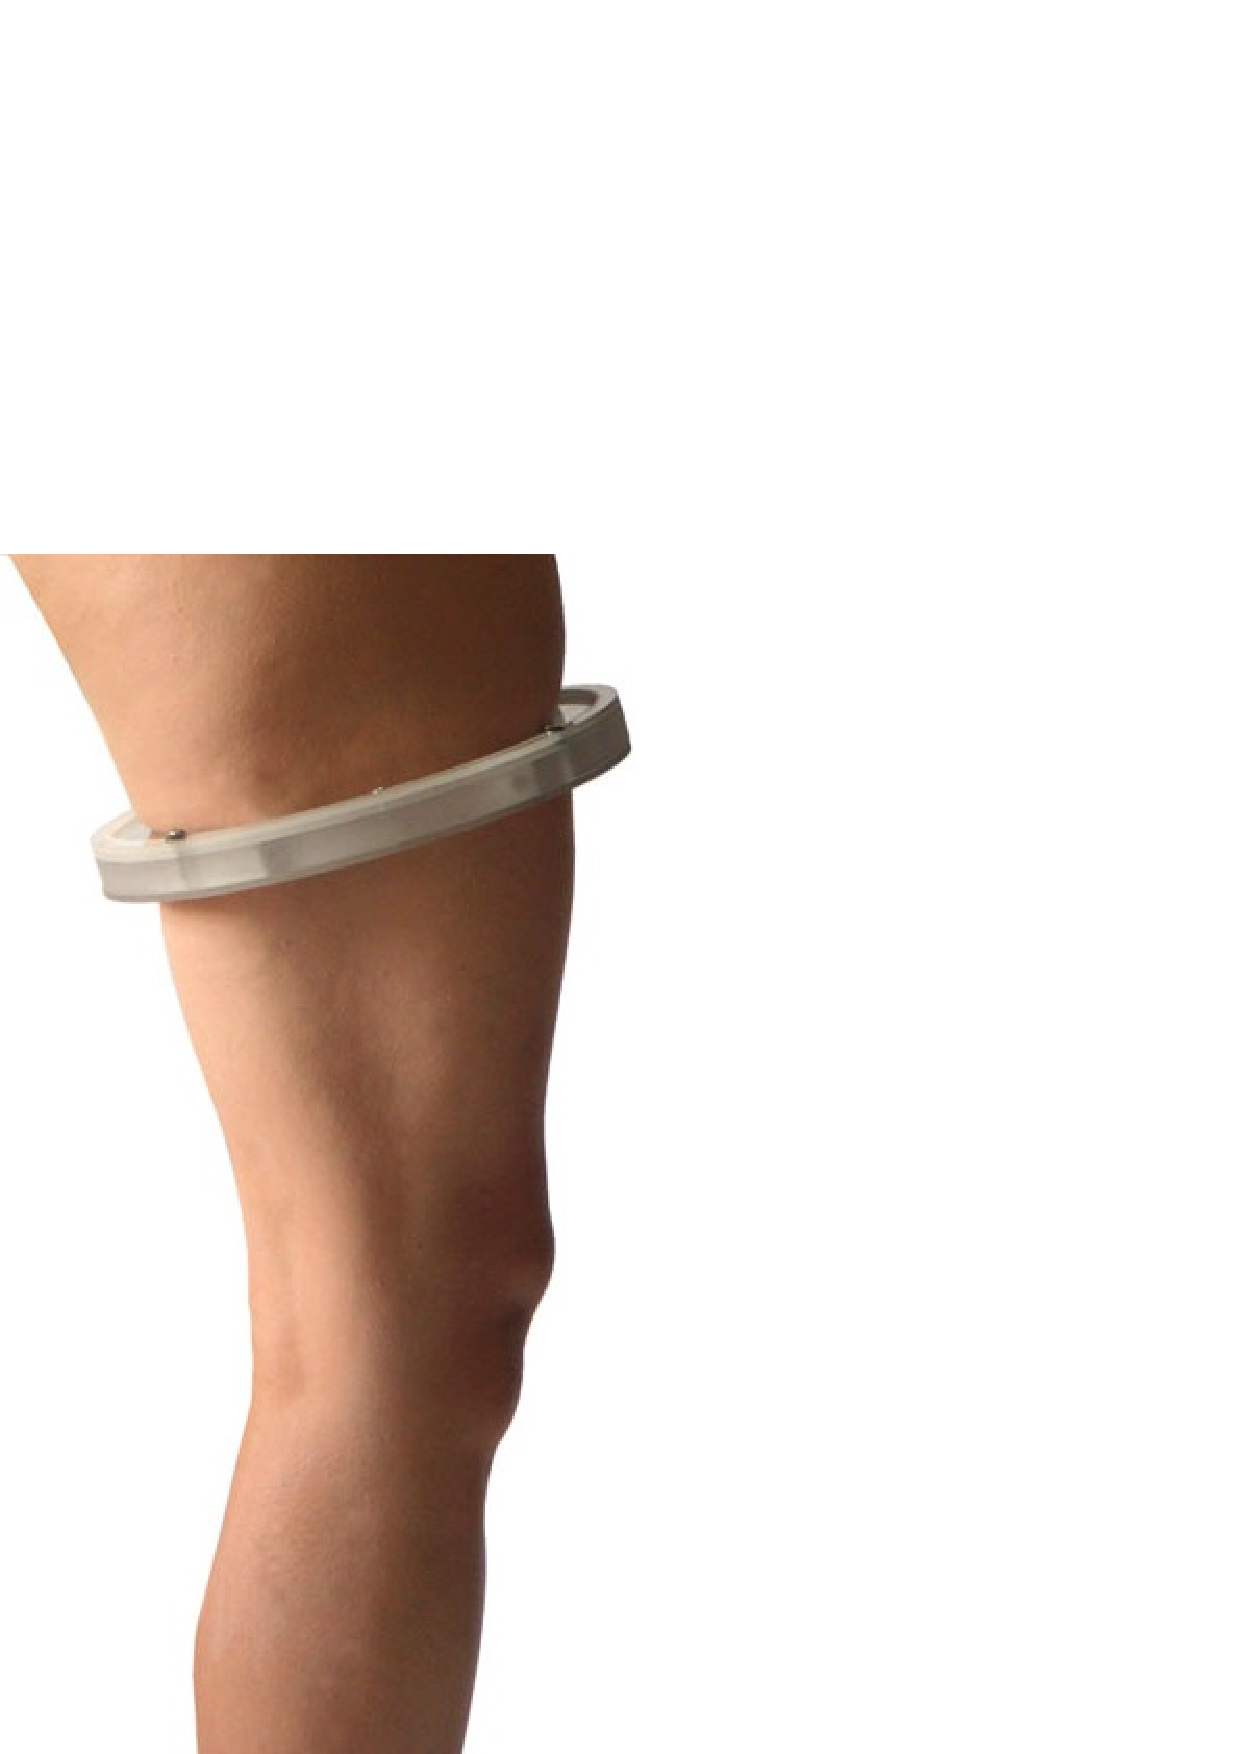
\includegraphics[height=2.5in]{thighmaster-leg}}
		\caption{Thighmaster energy feedback mortification device}
		\label{fig:thighmaster}
 	\end{center}
\end{figure}

R\"{u}st has implemented an extreme energy feedback system called the Thighmaster \cite{Rust2008Thighmaster-web}. Inspired by the cilice (a small metal garter with inward facing spikes) worn by some members of the Catholic Opus Dei organization as part of a practice of mortification, the Thighmaster is a ``techno-garter'' that pokes the wearer with spikes when their actions are not environmentally responsible (as defined by R\"{u}st), see \autoref{fig:thighmaster} for a depiction of the device. Specifically, the Thighmaster communicates wirelessly with electricity usage sensors and a human speech sensor that monitors whether the user speaks with their plants. While more of a demonstration, the Thighmaster shows the complex emotions involved in people's reactions to climate change. It goes without saying that being pierced by spikes is unlikely to be a viable energy feedback mechanism for most users.


\section{Motivation and Persuasion}

After making users aware of their carbon footprint, PET needs to persuade them to take actions to reduce their footprint, and motivate them to continue those actions indefinitely. Young investigated the motives behind individual's environmentally responsible behaviors (ERBs) through a series of surveys \cite{Young:2000fv}. Traditionally, the motives invoked by researchers attempting to promote ERB was constrained to material incentives or disincentives and altruistic reasons. The problem with incentives is that they ``needed constant reintroduction to remain effective and they proved to be less reliable than we had hoped''. Incentives can initiate ERB, but people's behavior changes back when the incentives end, and even continuing incentives can have low reliability.

Young also describes some of the pitfalls that can be encountered in motivating ERB, such as psychological reactance, where people do the opposite of the ERB they are being asked to undertake. Those initiating behavior changes can also be negatively impacted, creating feelings of contempt for those whose behavior is changing, and self-contempt.

Self-interest generally considered cause of environmental problems, ``focusing 
solely on short-term individual or familial gain to the exclusion of long-term societal or environmental benefits'', but Young suggests that self-interest can be a solution to environmental problems. He distinguishes self-interest from selfishness, self-interest meaning each individual is responsible for getting their own needs met. Young believes that intrinsic satisfaction is a better way to motivate ERB, as people find that ``certain patterns of behavior are worth engaging in because of the personal, internal contentment that engaging in these behaviors provides.''

Based on 9 different studies of ERB across different populations and environmental focuses, the author found 3 intrinsic satisfactions:
\begin{enumerate}
	\item ``satisfaction derived from striving for behavioral competence''
	\item ``frugal, thoughtful consumption''
	\item ``participation in maintaining a community''
\end{enumerate}
Competence involves the enjoyment in completing tasks and solving problems, frugality is enjoyment from the ``careful stewardship of finite resources'', and 
participation is the enjoyment from participating in community activities such as sharing news and collaborating with others toward a shared goal.

While attitudes and norms can lead to behavior change, people also need skills and experience with the change. As Young puts it, ``without considering these variables, we make the error of assuming that once people know what they should do and why they should do it, they will automatically know how to proceed.'' In the particular case of competence as a motivator, it is important to provide people with the opportunity to utilize their competence or they will grow frustrated. He suggests that motivating through competence be done by providing an environment where information on procedures is available and new behaviors can be tried out in a supportive environment.

Darby's survey of electricity feedback programs found similar results on motivations \cite{darby-review-2006}. She found that incentives to save energy lead to savings that disappear when the incentives are removed. When trying to get people to change their behavior, she found that behavior formed over a 3 month period is more likely to persist than those behavior changes made over shorter periods. She also found that internal motivation is most important for continuing energy savings.

In a position paper, Khan and Canny suggest that the technique of social marketing would be helpful in persuading users to make environmentally beneficial changes \cite{Khan2008-social-marketing}. Social marketing is the idea of applying the principles of consumer product marketing to encourage social change. The principles they describe are: emphasis on the benefits of new behavior while minimizing the cost, consumers are strongly influenced by knowing what behaviors others are undertaking, and target audiences should be segmented with different messages to different segments. For example, in discussing the iamgreen application (see \autoref{iamgreen}) where users commit to positive environmental actions suggested by others, the authors suggest using collaborative filtering (the technique used by online merchants to suggest other products similar to the one being viewed) to suggest leaves rather than just popularity.

\section{Design of Environmentally Persuasive Systems}

Considerable research has been done on the subject of designing environmentally persuasive systems. Woodruff et al performed a qualitative study of individuals who are making a significant effort to be green, in an effort to inform future designs by documenting existing green practices and beliefs \cite{Woodruff2008-bright-green}. The participants were all involved in making their home more sustainable and energy efficient, and that was the focus of the study. The authors found that these environmentally inspired people have diverse affiliations, and traditional environmental activism isn't always central to their interests. Thirty-five homes participated in the study, with 56 people in total. The participants were mostly ``bright green environmentalists'', that is environmentalists that believe that technology can make the world more sustainable, rather than believing that technology is the root of unsustainable behavior and should be abandoned. The authors divided the participants into three groups based on their motivations: ``counterculture bio-centric activism; American frontier self-reliance and rugged independence; and trend-focused utopian optimism.'' The first group focused on stewardship of the earth, the second group was focused on frugality, do-it-yourself activities, and patriotism from getting off foreign oil. The third group was focused on trend-setting, and being ``eco-chic''.

The authors found that the participants were reflective about the positive environmental choices they made, often trying to improve their sustainability through playful analysis of the options, such as buying a product online versus buying it from a store. They found that participants eagerly assessed the performance of their homes, so that they could tune them for better energy savings. This included extensive data collection, both manually and through automation. However, after living in a house for 1.5 years, their interest in data collection had gone down, in part because their routines had been internalized. In making their homes more efficient, the participants would work on improving one area at a time, then move on to the next area. Participants also wanted to live by example and inspire others, such as by driving a hybrid car.

Based on the interviews, the authors found several implications for design. The participants tended to learn about sustainability in a depth-based manner (focusing on one area at a time) rather than in a breath-based manner. Many popular attempts to encourage environmentally responsible behavior involve short lists of relatively easy actions, which is contrary to how the participants sought information. The authors suggest that advice systems focus on the user's primary motivations in-depth rather than providing a list of easy actions. The participants found mentorship an important part of the learning process, so the authors suggest that systems match mentees with mentors that have already mastered the area of expertise being sought. The authors suggest that users be provided with ways to express their identity and share their green activities to others via social networks. Finally, based on the observation that many participants enjoyed the process of determining the most sustainable option among many choices, Woodruff et al suggest providing users with modest mental puzzles that help users explore the outcomes of different actions rather than telling them the answer outright.

Darby's review of energy feedback studies yielded some suggestions for design \cite{darby-review-2006}. She observed that historical feedback of the user's energy consumption is more effective than feedback that compared usage to others, or feedback that compared usage to normative values. However, users did report finding pie charts of typical breakdowns of home energy use helpful, even though they were averages as opposed to being drawn from the user's data. Users reported that they liked to see comparative information, but that it didn't necessarily lead to energy savings. In addition, if a user is shown comparative data that indicates that their usage is lower than their peers, it could lead to the user feeling unconcerned about increasing their consumption to match their peers.

Chetty et al performed a qualitative study of the resource management processes of 15 households in an effort to help ubiquitous computing researchers design better resource feedback systems \cite{chetty-2008}. They found that participants were unaware of real-time resource consumption for both the entire home and individual appliances. The study examined the participants usage of natural gas, electricity, and water. Thermostats seemed to be a problem for participants, leading to arguments about how they should be set and half of the homes with programmable thermostats hadn't programmed them. Some participants were in living situations where they paid a flat rate for their utilities, which led to a lack of motivation to conserve resources. Participants wanted real time information on their resource usage, on utility pricing (if there is peak load pricing), and also alerts if there is anomalous usage (such as a broken toilet using an excessive amount of water). The authors report that participants were also aware of potential privacy issues, such as being able to infer other's habits from their resource usage, and feeling shame if one is wasteful with resources.

Based on their study, Chetty et al provide some suggestions for future system designs. In the modern world, infrastructure is invisible: you don't have to know how much energy an appliance uses when you plug it in. Therefore the authors suggest visualizations ``that equate our resource usage with units of production, for example, buckets of water, bags of coal, stacks of wood, as well as a monetary amount.'' They point out that households are often made up of multiple people with different levels of interest in being green and different responsibilities (some may not have to pay the bills!), so system design will have to reflect these differences. The authors also worry about the ``green divide'' in that lower income households might not be able to afford expensive equipment. They suggest the need to make sure devices supporting resource conservation are affordable to all.


\section{Related Systems}

In this section we examine other systems that have been designed to help users become more aware of their environmental impact. For more information on PET, the system I plan to build, see \autoref{PET-description}. Some of the sensors described in \autoref{sensor-section} could also be classified as related systems, since they provide feedback to the user. However, they are described separately as their emphasis is on the sensing. Carbon calculators can also be thought of as systems that make people aware of their environmental impact, but since they are numerous and narrow in focus they are described separately in \autoref{carbon-calculators}.

The system closest to PET is the one described in the position paper by Sutaria and Deshmukh \cite{sutaria-2008}. It describes using networks of ad hoc sensors to monitor both electricity usage and miles driven by automobile, while providing real-time feedback to the user. The system described would compare the household's energy usage with others in similar situations. They envision smart energy meters that can also provide suggestions on how users can reduce their energy usage. They also mention the possibility of integrating personal carbon trading (a sort of carbon cap-and-trade system for individuals) into the system, such as the one being investigated by the RSA CarbonLimited project \cite{carbonlimited-2007}. While the system described by Sutaria and Deshmukh is similar to PET, the system appears to be hypothetical at this point.

\subsection{StepGreen}

StepGreen is a web application designed to encourage people to undertake environmentally responsible actions \cite{step-green-website}. Mankoff et al have written about the rationale for the system and description of the design, presumably written before the site was active \cite{Mankoff2007Leveraging-Soci}. The basic idea is that half of American's consumption of energy is under their control, but people don't connect their activities with \COtwo emissions. StepGreen (also known as Footsteps, possibly an earlier name for the system) is designed to leverage online social networks to motivate personal change, by providing suggestions for improvement.

\begin{figure}[htbp]
	\begin{center}
		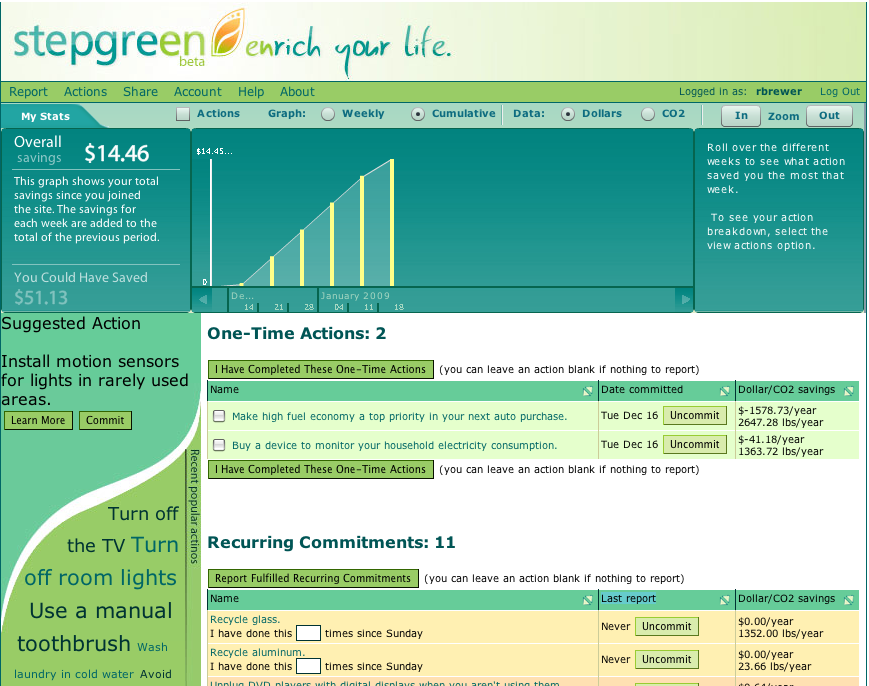
\includegraphics[width=\textwidth]{stepgreen-bitmap}
		\caption{Example page from StepGreen website}
		\label{fig:stepgreen-website}
 	\end{center}
\end{figure}

The StepGreen system is currently open to the public, \autoref{fig:stepgreen-website} shows an example of the default page shown when a user logs in. Users create an account on StepGreen, and then are presented with a list of actions with positive environmental consequences (mostly reduced GHG emissions). Example actions are ``Turn off the lights when you exit the house in the morning for the day'', ``Take the stairs at work'', and ``Set your home computer to automatically hibernate/sleep after a short period of inactivity''. Each action is associated with a cost savings and reduction in \COtwo emissions, and users can get more information about the action and how the savings were calculated. For each action, users can indicate whether they are already performing that action, whether they commit to undertaking that action, or whether the action is not applicable to them. The current system does not appear to have a way to suggest to actions to be added to the list, but based on the design paper \cite{Mankoff2007Leveraging-Soci}, this might be added at some time in the future.

Once users have selected actions that they are either already performing or commit to performing, they can track them on the Reporting page. For one time actions, such as replacing an incandescent light bulb with a compact florescent bulb, users simply check off when they are completed. For recurring actions, users must indicate how many times they have performed the action since their last report in order for the system to track the activities. Based on the user's self-reporting, StepGreen calculates the amount of money saved, pounds of \COtwo saved (i.e. reduced), and missed pounds of \COtwo saved, and provides a historical graph of values.

StepGreen also provides links to social networking sites. They provide a linked Facebook application, a MySpace profile widget, and connection to Twitter. Each of these links provides a way to inform the user's social network about what actions the user is undertaking. This can serve to recruit other people to use StepGreen, provide comparisons on financial and environmental savings between peers, and encourage users to keep to their StepGreen commitments. 

StepGreen provides a useful platform for research on convincing users to change their behavior to reduce their carbon footprint. For example, a virtual polar bear was implemented to motivate users to reduce their carbon footprint (see \autoref{virtual-polar-bear}). Notes on the StepGreen research website \cite{stepgreen-research-website} indicate that there are plans to support the input of sensor data from the UbiGreen transportation sensing project that they are a part of (see \autoref{ubigreen}).

In its current state, StepGreen would be challenging to keep up to date due to the reliance on manual data input. The actions available in the system are quite wide-ranging, but focus on relatively minor changes such as not using an electric toothbrush. Without the overall view that PET intends to provide, it would be easy to focus efforts on these minor actions instead of tending to the major sources of one's carbon footprint. Due to the limitations of manual reporting, StepGreen may report missed savings that are not accurate, annoying users. For example, recycling glass is an action that is listed as having substantial carbon savings. However, if one chooses to drink water from a mug instead of purchasing a beverage and later recycling the glass container, clearly the carbon savings are greater from using the mug, but StepGreen will count the lack of recycling as missed savings. PET is designed to work from sensor data primarily, which should reduce the issue of inaccurate missed savings. PET's data focus could also allow it to improve on StepGreen's action list by suggesting actions that are directly address the user's largest sources of carbon emissions.

\subsection{Virtual Polar Bear}
\label{virtual-polar-bear}

Dillahunt et al (who are involved with the StepGreen project) have built a system providing a virtual polar bear that is affected by the user's environmental choices as a means to motivate users to reduce their carbon footprint \cite{dillahunt-virtual-polar-bear-2008}. They note that there are strong emotional bonds between humans and animals, which may help to encourage environmentally-responsible behavior. The authors performed a one week study, with subjects divided into two groups: an attachment group and a control group. The attachment group read a story about climate change impacting polar bear habitats, and were asked to name their virtual polar bear. As participants make or decline commitments to environmentally responsible actions, the ice under polar bear either grows or shrinks (see \autoref{fig:virtual-polar-bear} for images of the polar bear). The study had 20 subjects (10 for each group), all of whom were surveyed before and after to test for levels of empathy and environmental concern. The subjects in the attachment group had more fulfilled environmental commitments, which was a statistically significant difference. The attachment subjects also had a greater level of environmental concern after interacting with the polar bear. The study was short, so the authors are unsure whether effects would be sustained in a longer study. They are now working on bringing the system to a mobile platform and a polar bear application for Facebook and MySpace.

\begin{figure}[htbp]
	\begin{center}
		\includegraphics{virtual-polar-bear}
		\caption{Example images of virtual polar bear with lots of ice and with little ice}
		\label{fig:virtual-polar-bear}
 	\end{center}
\end{figure}

\subsection{iamgreen}
\label{iamgreen}

iamgreen is an application for the Facebook social networking platform that provides an online gathering place for environmentally conscious users \cite{iamgreen-website}. iamgreen provides all of the standard components of Facebook: a newsfeed of events from members, status updates, news articles, etc. The application provides a list of environmentally responsible statements called leaves, such as ``Most of my lightbulbs are compact fluorescents'', ``I recycle, even when it is not convenient'', and ``When I drive, it's over 40mpg baby'' (see \autoref{fig:iamgreen} for an example of the leaf selection page). Users can indicate for each statement that they engage in that behavior, they aspire to that behavior, they wish to hide the statement (removing it from the list of choices), or they want to recommend it to a friend. Users can then display the number of leaves they have committed to in their Facebook profiles. Users can also contribute new leaves that will be displayed as options to other iamgreen users.

\begin{figure}[htbp]
	\begin{center}
		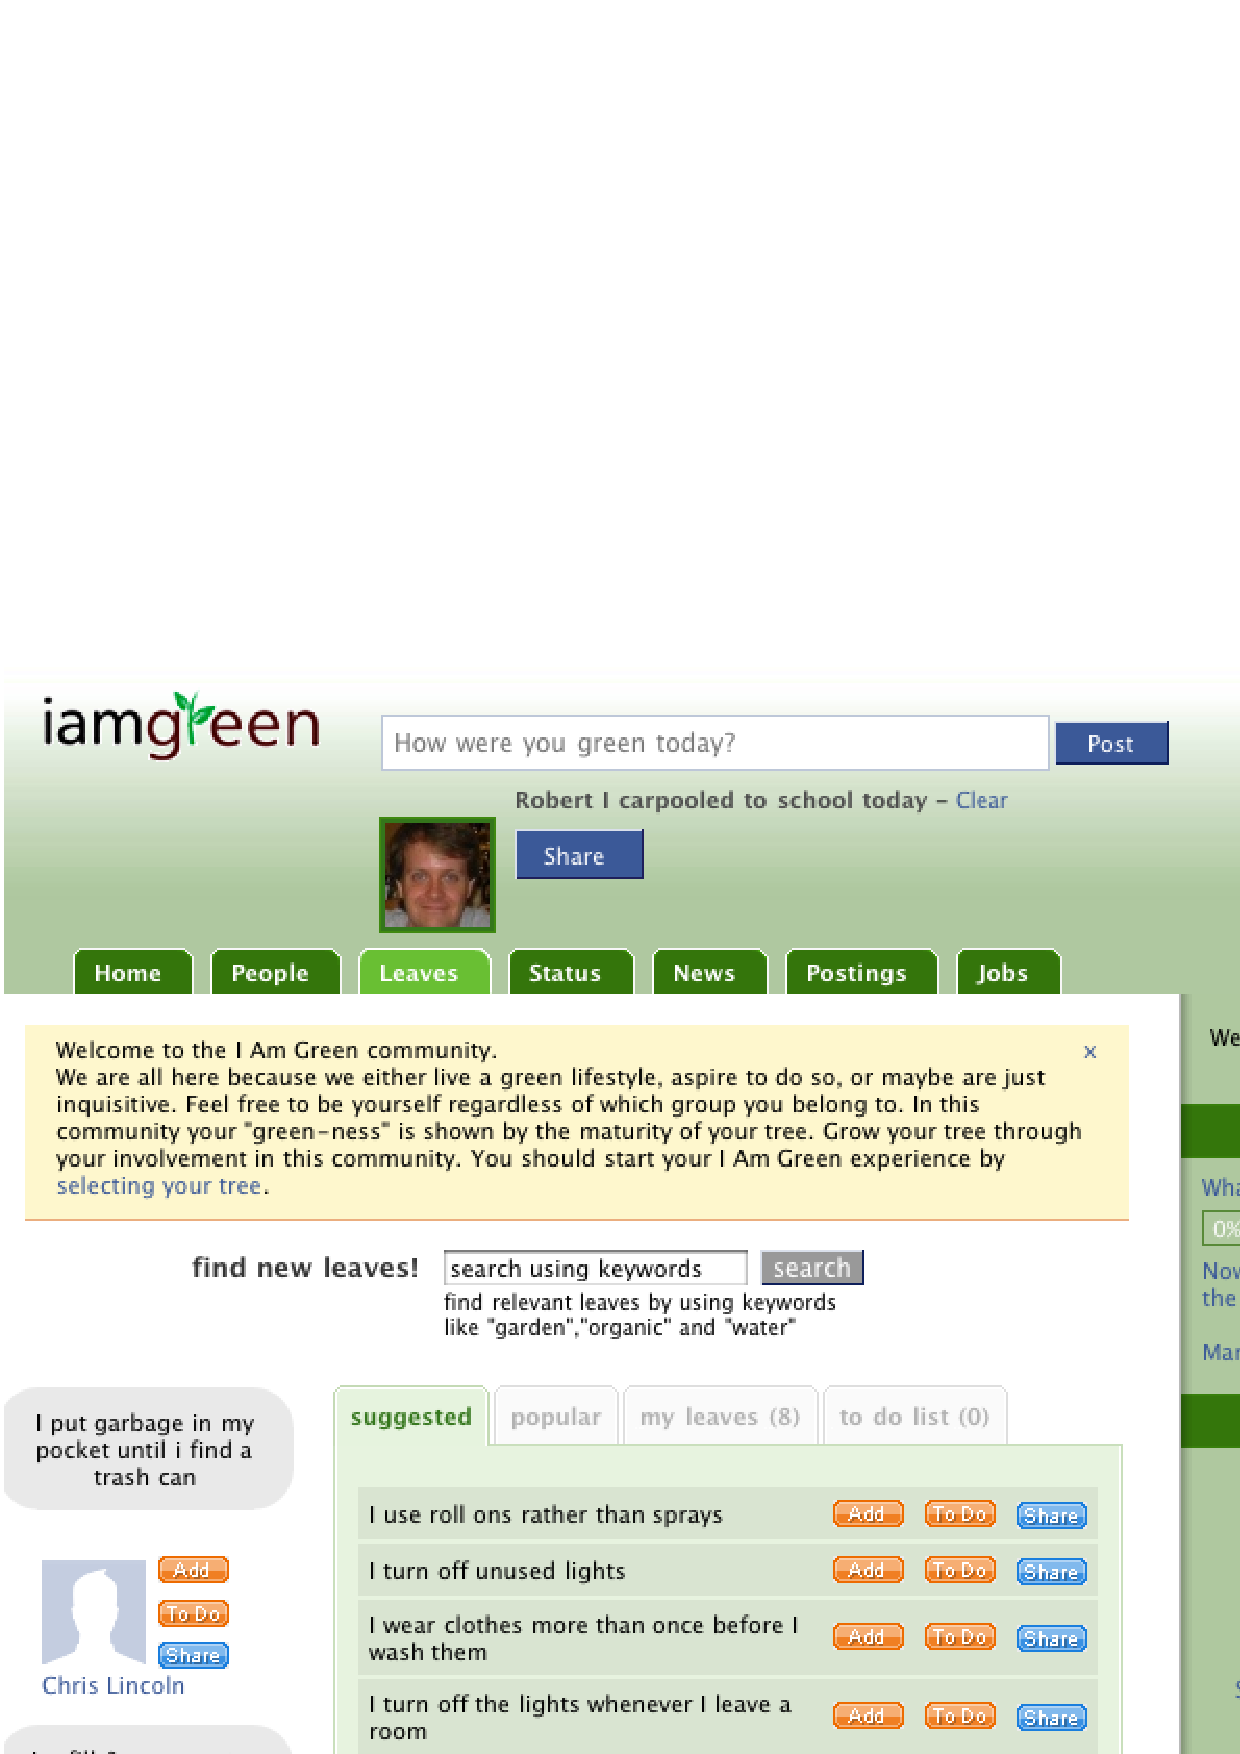
\includegraphics[width=0.8\textwidth]{iamgreen}
		\caption{Leaf selection page of iamgreen Facebook application}
		\label{fig:iamgreen}
 	\end{center}
\end{figure}

While the leaves concept is a simple way to encourage users to make more environmentally positive choices, it suffers from some obvious deficiencies. First, leaves have mostly the same value (though apparently some actions, such as not owning a car, are worth more than one leaf). The leaf system also lacks any quantitative feedback other than the number of leaves, so the user is not provided with real insight into their environmental footprint. Like any system based on manual reporting, users have to spend time reporting any changes to their action list. Without quantitative feedback, it seems likely that many users will make some selection of leaves and then revisit them infrequently or never again.

\subsection{Personal Environmental Impact Report}

Personal Environmental Impact Report (PEIR) is a mobile phone sensing-based environmental data collector from the urban sensing group at the University of California, Los Angeles Center for Embedded Networked Sensing (CENS) \cite{peir-website, agapie-2008-seeing-our-signals}. The PEIR application runs on GPS-enabled mobile phones to record users' locations throughout the day. The data is uploaded to a central server that provides each user with a profile of their environmental data. Unlike most applications, PEIR not only tracks the user's impact on the environment through GHG emissions, it also tracks the environment's impact on the user. PEIR currently tracks the user's carbon emissions, their contribution to pollution around schools and hospitals, their exposure to fast food establishments, and their exposure to fine particulate matter in the air. The sensed data is overlaid on a map that allows users to see the location of problematic areas (primarily useful for seeing the user's exposure to particulate matter). \autoref{fig:peir} shows the PEIR web interface. PEIR also provides a Facebook application that shows the user's current environmental impact, and ranks the user against their friends impacts.

\begin{figure}[htbp]
	\begin{center}
		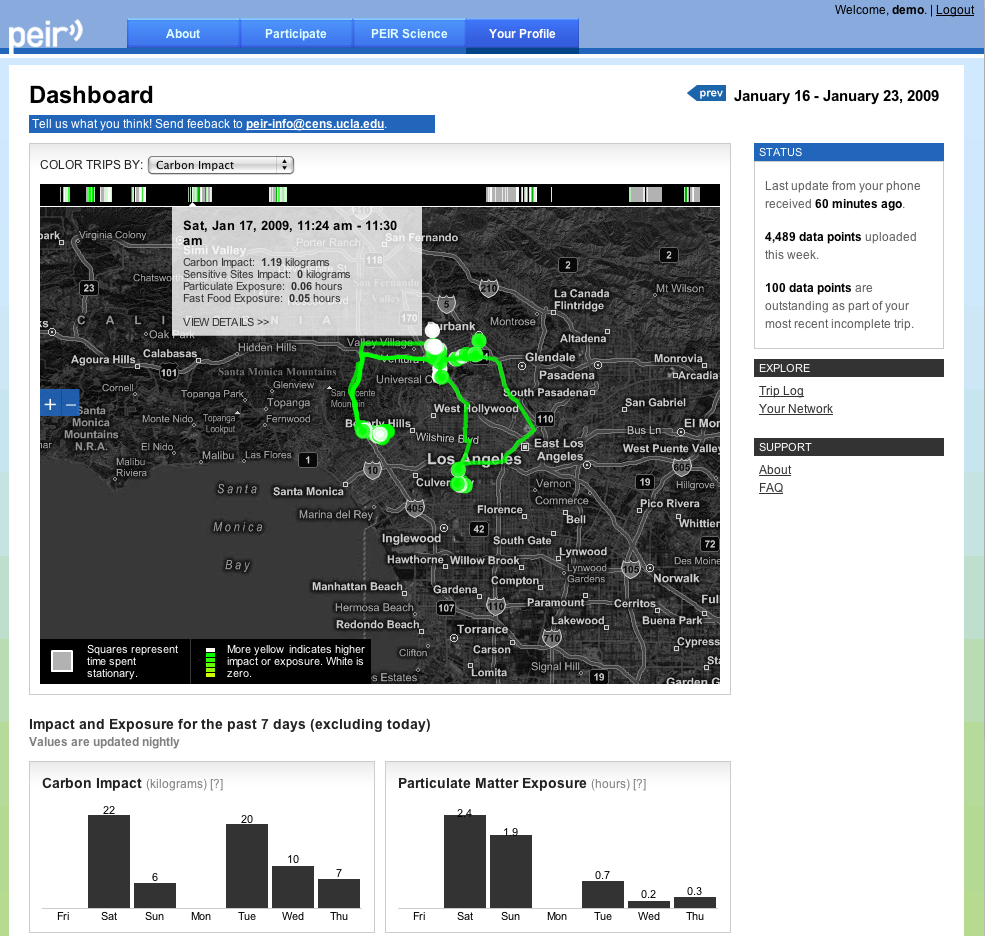
\includegraphics[width=\textwidth]{peir-bitmap}
		\caption{PEIR Dashboard web page showing recent trips and associated footprints}
		\label{fig:peir}
 	\end{center}
\end{figure}

The only data the PEIR system directly measures is the user's location at a particular time. From the location data, activity inference is done by matching locations to freeway data from maps, and the speed from GPS location data. These are combined using a Hidden Markov Model to infer if the user is still, walking, or driving. The location and activity data is combined with GIS, weather, and environmental information such as smog levels to produce the information on the four impacts listed previously.

As of this writing (December 17, 2008) PIER is in a closed beta test, so it is not available to the public yet. It currently runs on the Nokia N80 with external GPS device or the Nokia N95 with built-in GPS, with plans to accept GPS traces from arbitrary sources (such as GPS data loggers) in the future.

PEIR is an impressive system, incorporating location sensor data and extensive analysis to provide four very different impacts. The project is currently focused on transportation-related environmental impacts because people have  choices in meeting their transportation needs, but the developers indicate that they will add sensors from other domains in the future. Currently the system only provides measurement data, and doesn't make any attempts to change users behavior. While the fast food exposure measure is cute, it isn't quite parallel to the other impacts since it is possible to not patronize fast food establishments in one's vicinity, but ones exposure to fine particles cannot be willed away.

\subsection{mobGAS}

mobGAS is mobile phone application that computes GHG emissions from a detailed, manually-entered daily diary of activities \cite{mobGAS-website}. The data entry is quite detailed, including: transport, appliance use, lighting, heating/cooling, hygiene, and food (see \autoref{fig:mobGAS} for an example data entry screen). The results can be uploaded to a central server where they can be reviewed by the user, or used to generate a ranking of all users. The system was designed for use in the European Union: only EU countries can be selected when registering an account,  so it cannot accurately calculate GHG emissions for people living in the US.

\begin{figure}[htbp]
	\begin{center}
		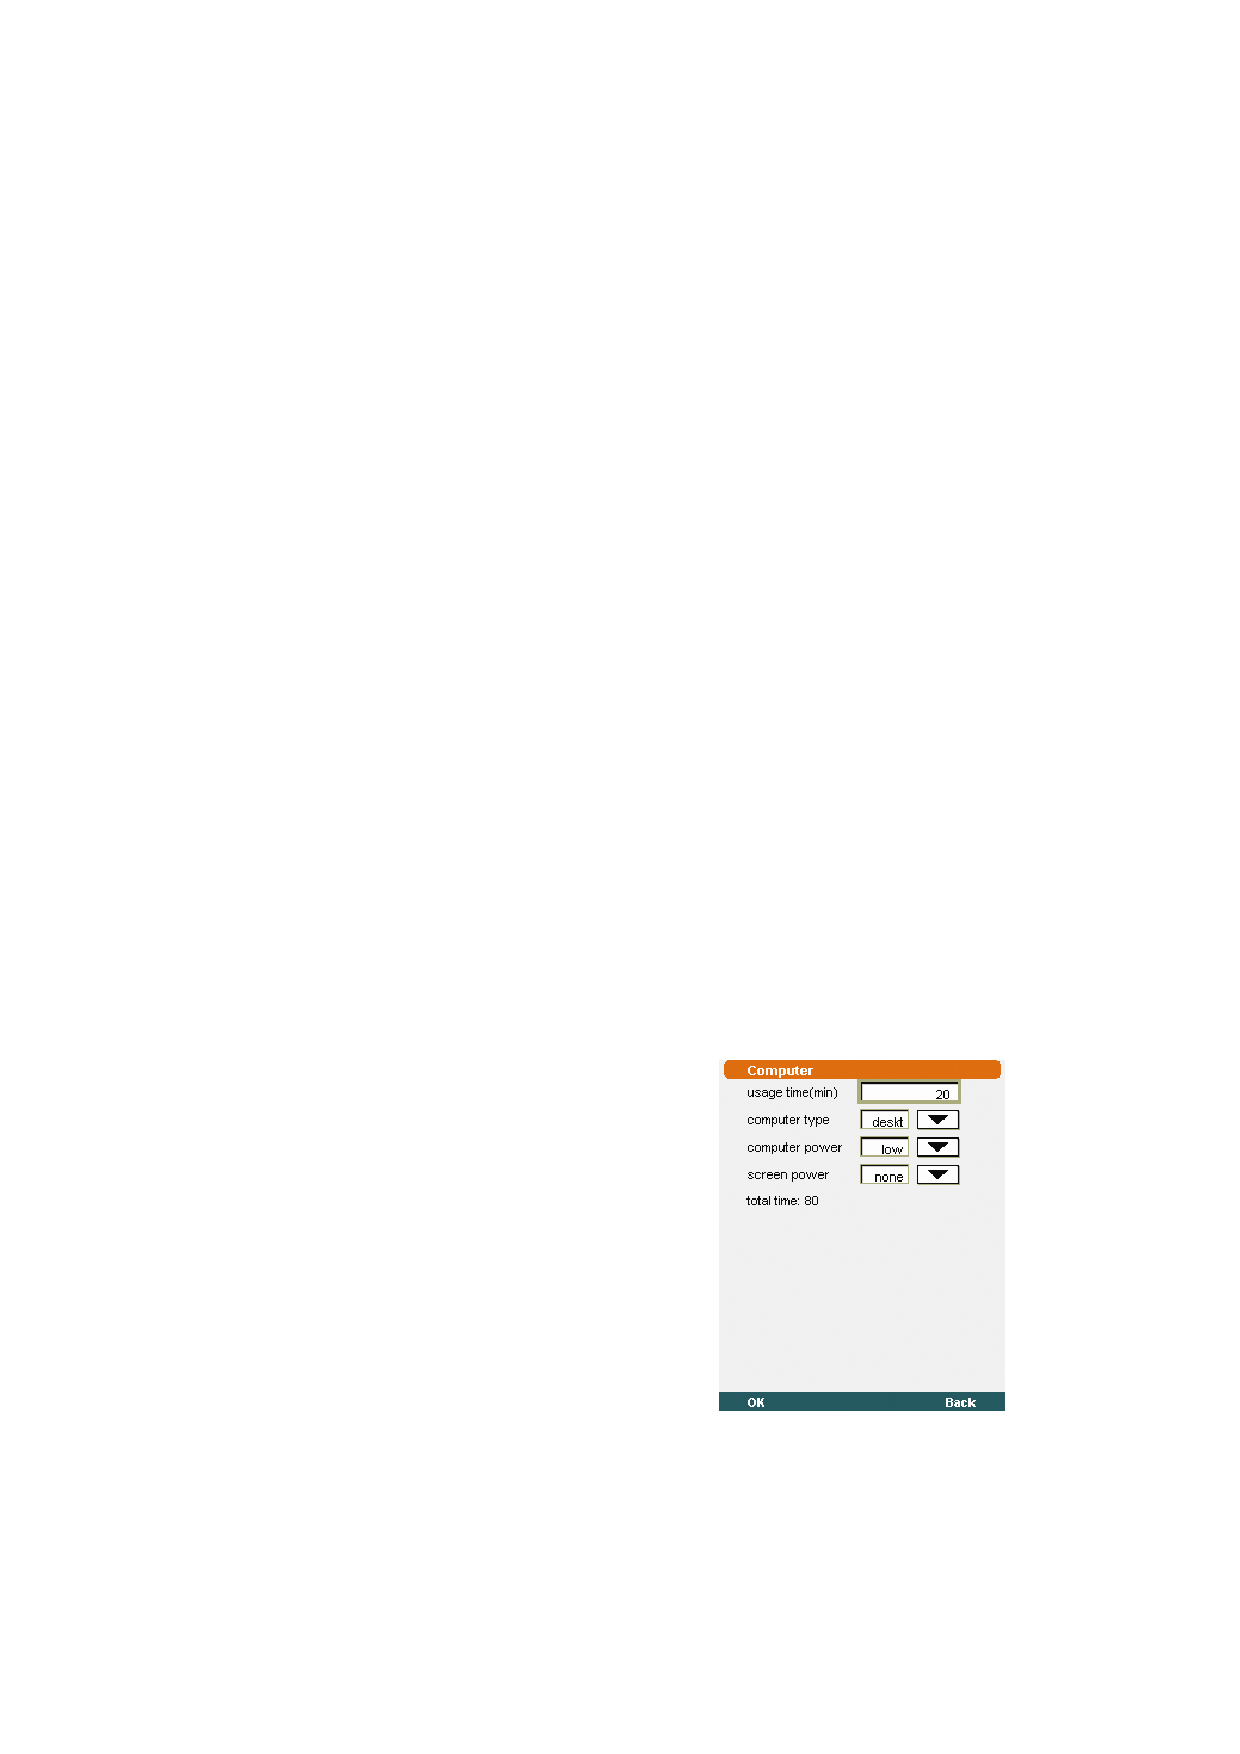
\includegraphics{mobGAS}
		\caption{mobGAS application showing a data entry screen for computer usage}
		\label{fig:mobGAS}
 	\end{center}
\end{figure}

On November 25, 2008, the user ranking page\footnote{\url{http://mobgas.jrc.ec.europa.eu/mobgas/app/emissions/userrankings.po}} shows only one user ``Galloz'' who has 0.65 kg of GHG emissions. So either the ranking page is not working properly, or there is one actual user of the system, who has entered in very little data (or perhaps lives as a hermit).

The team behind mobGAS has released a ``disclosed model'' report that explains both the functionality available in the program and the model used to compute the GHG emission information \cite{Sousa-Pedrosa2008mobGAS-model}.

While attempting to capture GHG emissions from a wide range of activities is admirable, it seems unlikely that people will enter such detailed data manually on a regular basis. Even if users were so inclined, the mobile phone environment is far inferior to a desktop or laptop computer for data entry.

\subsection{Personal Kyoto}
\label{personal-kyoto}

Personal Kyoto is a web service that tracks the electricity usage of users in the New York area, and compares it to a ``Personal Kyoto Goal'' for the user \cite{Personal-Kyoto-website}. The Personal Kyoto Goal represents the limit of electricity usage that would apply to the user if the Kyoto Protocol (which the USA is not a party to) were administered on an individual basis rather than on a national basis.

The user's electricity usage is retrieved from the local utility's web site (Con Edison) using the user's account number. In addition to the monthly usage (which can vary substantially due to circumstances and the seasons), a 12 month rolling average is computed to remove the seasonal effects. The Personal Kyoto Goal is defined as 75\% of the first point of the monthly moving average when the user signed up with the web site. \autoref{fig:personal-kyoto} shows an example graph with monthly averages and a personal Kyoto goal.

\begin{figure}[htbp]
	\begin{center}
		\includegraphics[width=\textwidth]{personal-kyoto}
		\caption{Example graph of electricity usage from Personal Kyoto}
		\label{fig:personal-kyoto}
 	\end{center}
\end{figure}

Personal Kyoto is a cleverly designed system in that it uses the user's real data, but avoids manual data entry by scraping the data from the utility web site. It also gives the user a specific goal for reducing electricity use that has a real justification and ties into the environmental ``gravitas'' of the Kyoto Protocol.

\subsection{EcoIsland}
\label{ecoisland}

Takayama and Lehdonvirta have constructed a system they call EcoIsland, which attempts to ``motivate behaviour changes that reduce CO2 emissions'' using a background game-like activity, with a centrally installed display in the home \cite{takayama-2008} (see \autoref{fig:ecoisland} for an example of the user interface). Each family member has an avatar on the virtual island, and they set a family \COtwo emissions target. The family's emissions are tracked via sensors and self-reporting. If the emissions exceed the chosen target level, the water level on the island rises, and if the water level continues to rise it will eventually end the game.

\begin{figure}[htb]
	\begin{center}
		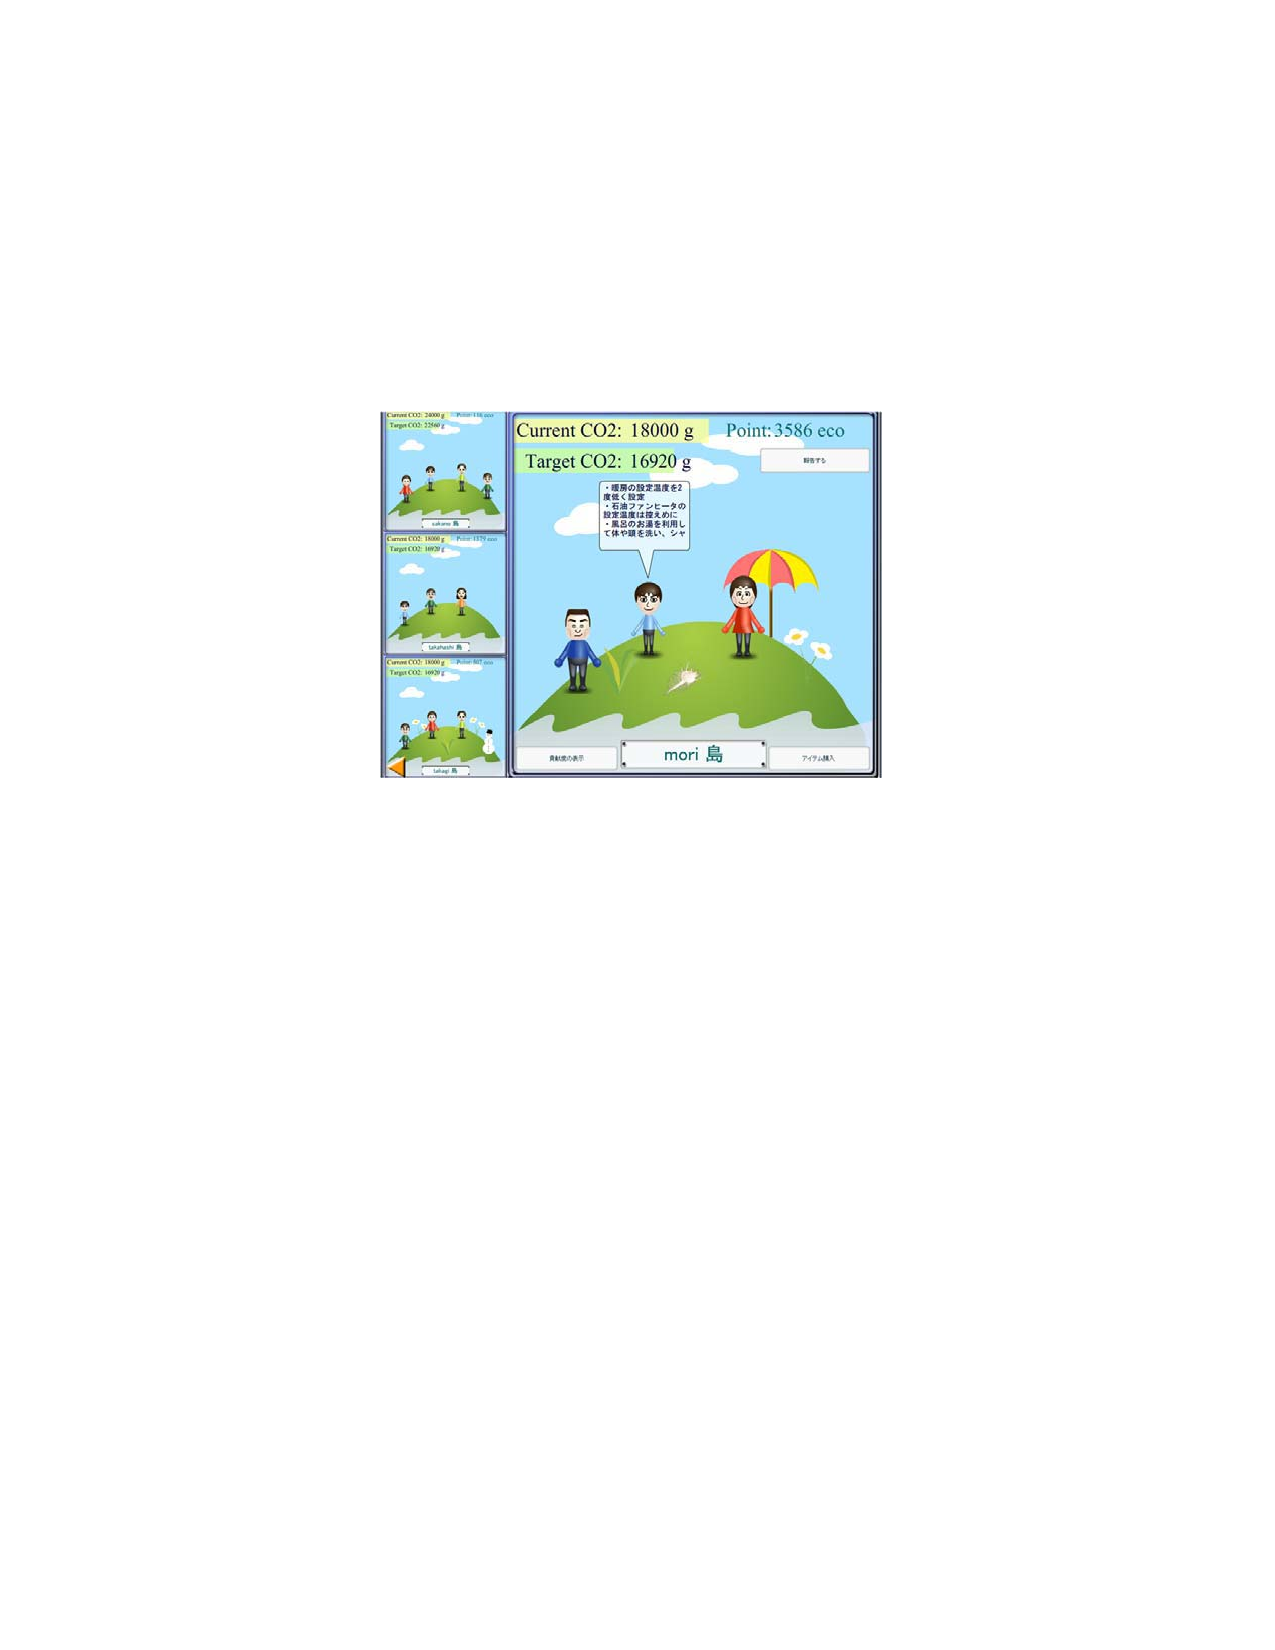
\includegraphics[width=0.8\textwidth]{ecoisland}
		\caption{Example EcoIsland display, with family avatars}
		\label{fig:ecoisland}
 	\end{center}
\end{figure}

Participants mobile phones have a list of suggested actions to reduce emissions, and they can self-report their actions using the phone. Participants can see the islands of other participants and they receive a periodic allowance in a virtual currency. The participants can use the virtual currency to buy decorations for their island, or they purchase carbon credits from other users. Therefore participants with low emissions can decorate their island, but those with high emissions have to spend their money on carbon credits. EcoIsland provides a metaphor for the users' emissions and makes them aware of the consequences of their actions.

At the time of the paper's writing, the sensor portion of the system was not yet implemented. The authors performed a four week pilot study of EcoIsland with 20 people in six families. During the first week, the baseline electricity usage of each participant's air conditioning system was monitored using a plug load meter (for more information on this type of meter, see \autoref{plug-load-meters}). During the second week, one participant from each household was asked to use the system, while in the third week all members were asked to use it. In the fourth week, the carbon trading system was introduced to participants. At the conclusion of the study, the participants were surveyed and 17 of 20 participants said ``they were more conscious of environmental issues after the experiment than before.'' However, users indicated that they were motivated by game issues (such as saving the sinking island and buying decorations) rather than saving the environment. Few of the participants used the carbon trading system because their targets were easy enough to achieve without trading. Air conditioner usage in participant homes showed no correlation with game outcome, but the authors believe that the short study, conducted in winter [sic!] may have affected that outcome. One interesting result is that participants noted that manual reporting contributed to their motivation, so replacing the reporting with sensors could reduce user's motivation to change.

\subsection{Dopplr}
\label{sec:dopplr}
Dopplr is a web application for organizing travel plans and coordinating ad hoc meetings with friends who are also travelling \cite{dopplr-website}. Users enter in their travel plans by specifying one or more destinations and the mode of transportation used for each leg of the trip. Dopplr has an index of place names, so users can easily type in the name of each city they are visiting and Dopplr will figure out where each city is located. The system can also parse e-tickets and itineraries forwarded via email, reducing the amount of manual input required.

\begin{figure}[htb]
	\begin{center}
		\includegraphics[width=0.85\textwidth]{dopplr}
		\caption{Example of Dopplr's carbon footprint calculations}
		\label{fig:dopplr}
 	\end{center}
\end{figure}

Dopplr is also a social network where users can share their travel plans with each other. If two friends happen to be in a particular city at the same time because their travel plans intersect, Dopplr will notify both users so they can decide if they want to meet up.

Dopplr now provides each user with a carbon footprint calculated from their trip data. The calculations are done using AMEE (see \autoref{amee}), which uses the distance of each leg and the mode of transportation to compute the number of kilograms of \COtwo emitted by each trip. \autoref{fig:dopplr} shows an example of Dopplr's carbon footprint display.

From PET's perspective, Dopplr is more of an information sensor that leverages information that users record about themselves. In particular, the primary goal of Dopplr users is sharing travel plans with their social network, and the carbon calculation is just a convenient analysis that can be performed with the same data.

Dopplr provides an API for developers that wish to extract information about a user's travel plans programmatically. Unfortunately, at this time (December 2008) the API does not allow retrieval of the carbon data. However, the trip information is available from the API, so the calculations themselves could be done outside of Dopplr (potentially even using AMEE). Carter has created a website that calculates the carbon footprint of a user's entire Dopplr social network using this general technique \cite{offsetr-website}. Another limitation of using Dopplr for calculating air travel carbon footprints is that Dopplr generally only records the user's final destination, not the series of flights required to get to the destination. Since many long plane trips involve one or more legs, Dopplr underestimates the carbon footprint by using the (always less than or equal to) direct distance between the start and finish cities. Since Dopplr is designed around social connections, this limitation makes sense because users are unlikely to be able to meet friends between flights.

\subsection{Related Systems Summary}

The systems here represent a diverse set of methods for monitoring and encouraging the reduction of users' environmental footprint. \autoref{tab:related-work-synthesis} summarizes the systems reviewed. The columns of the table are:

\begin{itemize}
	\item Data input: the means by which data about users' activities are input into the system. The options here are: \emph{physical sensors} (such as GPS or ammeters), a list of \emph{green actions} (like turning off lights after leaving a room), \emph{manual} input (typing in the number of miles driven), or \emph{information sensors} (grabbing data already online, like electricity usage from a utility website).
	\item Social aspect: what social functionality the system provides, if any.  The options here are: a \emph{social networking plugin} (for a site such as Facebook or MySpace), a \emph{user ranking} based on some green criterion, \emph{collaboration} facilities such as a discussion forum or suggesting green actions to others, or social interaction is \emph{integral} to the system (without it the system wouldn't work).
	\item Suggestions: does the system provide suggestions to the user on how to reduce their environmental footprint?
	\item Interface: how do users interact with the system, with the primary mode of interaction listed first. The options are: a \emph{website}, a \emph{mobile phone} application (or a website tailored for mobile browsers), or some sort of \emph{custom display} (such as an energy meter that displays a home's current electrical usage).
	\item Status: the status of the system. The options here are: the system is \emph{proposed} (it only exists on paper), the system is a \emph{prototype} (it works well enough to allow some sort of evaluation, but is not fit for wider use), the system is actually working but only in a \emph{closed beta} test, or the system is open to the \emph{public}.
	\item Leverage: what way, if any, could PET leverage this system to reduce the amount of implementation effort required? The options are: \emph{data input} (providing some way to directly input data in bulk), \emph{data output} (providing a way to export data that has been collected), \emph{API} (providing programmatic means to operate the system), and \emph{source code}. Note that some of these options are not supported by any of the systems reviewed.
\end{itemize}

\begin{table}[htbp]
	\begin{center}
		\begin{minipage}{\textwidth}
		% need small font sizes to make table fit on page
		\scriptsize
		\begin{tabular}{| l || p{2cm} | p{2cm} | l | p{2.25cm} | l | p{1.5cm} |}
			\hline
			System & Data Input & Social Aspect & Suggestions & Interface & Status & Leverage \\ \hline \hline
			
			Sutaria \& Deshmukh & physical sensor & user ranking, collaboration & yes & custom displays \& website? & proposed & N/A \\ \hline
			
			StepGreen & green actions & social network plugin & yes & website & public & none \\ \hline
			
			Virtual Polar Bear & green actions & none & no & website + Flash & prototype & none \\ \hline
	
			iamgreen & green actions & integral & yes & website & public & none \\ \hline

			PEIR & physical sensor & social network plugin, user rankings & no? & website & closed beta & data input (future) \\ \hline

			mobGAS & manual & user ranking & no? & mobile \& website & public & none \\ \hline

			Personal Kyoto & info sensor & none? & no & website & public & none? \\ \hline
%\footnote{Unable to verify without ConEdison account}
			EcoIsland & manual \& physical sensor & integral & yes & custom display, mobile phone & prototype & none \\ \hline

			Dopplr & manual \& info sensor & social network plugin, collaboration & no & website & public & API \\ \hline
			
		\end{tabular}
		\end{minipage}
	\caption{Systems related to PET}
	\label{tab:related-work-synthesis}
	\end{center}
\end{table}

Dopplr provides the best leverage for PET, as it provides a public API that would allow it to be used for collecting air travel sensor data. Unfortunately, none of the other systems provide any significant leverage for PET. The closest is PEIR, which claims that it will at some future time allow raw GPS to be uploaded for analysis, but without a means to extract carbon footprint data it is not useful for PET. The publically-available systems so far only provide lists of green actions as input, which is poses significant problems for user adoption. Several of the systems provide suggestions for change to the user, but none of them are tailored to the user based on past behavior or data.


\section{Sensors}
\label{sensor-section}

Integral to the PET concept is input from a diverse set of sensors. This section describes different types of sensors that relate to PET's mission to inform users about their environmental impact. Some of them are potentially data sources for PET.

\subsection{Electricity Usage}

Electricity usage is one of the major sources of GHG emissions for individuals, so being able to track its usage is a high priority. Electricity metering systems can be broken down into two types: plug load meters that measure the electrical load directly plugged into them, and whole home energy meters that measure the electrical usage of an entire home. Both typically provide a real-time display of electricity usage, and some sort of historical total (usually in kilowatt hours, kWh).

\subsubsection{Plug Load Meters}
\label{plug-load-meters}

The Kill-A-Watt (sold by P3 International) is an example of an inexpensive plug load meter \cite{kill-a-watt}. It is designed to be plugged into a wall outlet, and the load is then plugged into the Kill-A-Watt. An LCD display shows the current voltage, current, power, frequency, power factor, and cumulative energy used since the unit was plugged in. The Kill-A-Watt provides an easy way to determine how much electricity a particular appliance (or set of appliances if connected via a power strip) uses. The manufacturer claims the Kill-A-Watt has 0.2\% accuracy. There are several drawbacks to the Kill-A-Watt. Because of its shape, it generally obscures both of the outlets commonly found on a wall outlet in the US, preventing the second outlet from being use while measurement is taking place. The load most be plugged in via the Kill-A-Watt, so that means that the user must disconnect the load from power at least momentarily, which can be inconvenient for some loads (computers, VCRs, etc). The Kill-A-Watt also has no facility for exporting the data it collects, and if power is lost for any reason, the data collected will be lost as well.

LeBlanc attempted to address the issue of data collection with his work on recording device-level power consumption \cite{leblanc-2007}. He developed a sensor that sits between the load and the wall outlet, like the Kill-A-Watt. The sensor records electricity usage, and transmits the data wirelessly using the ZigBee protocol to a base station. Details on how to construct the wireless power monitor can be found at the author's personal website \cite{LeBlanc2008power-mon-howto}. This system solves the problem of automated data collection, but still requires the load to be unplugged before monitoring. It also faces the problem of all plug-load meters, that it can only monitor what it is connected to, so it doesn't work well for providing a comprehensive picture of electricity usage in a home.

\subsubsection{Whole Home Meters}
\label{whole-home-meters}

The Energy Detective TED Model 1001 is a whole home electricity meter from Energy, Inc \cite{the-energy-detective}. TED consists of two portions: a base unit that is connected directly to the incoming power lines at the circuit breaker box, and a display unit that connects to any power outlet in the home. The base unit uses current transformers that clamp over the incoming power cables and measure the amount of current being transmitted over them. Since the transformers clamp over the existing cables, there is no need to alter the existing wiring. The instantaneous power consumption can be computed using the current data combined with the utility voltage. This data is transmitted to the display unit through the home's electrical wiring.

Once the display unit is plugged into any outlet in the home, it receives the instant power consumption data from the base unit once a second. The power consumption data can be displayed in real-time in kW or dollars (after the user enters pricing data). It can also track historical consumption, peak usage, and project usage for the rest of the month based on historical usage. With the addition of the Footprints software package from Energy Inc, the display unit can be connected to a computer via USB to graph and record the data in a variety of formats. Energy Inc makes an API available for developers that wish to use the data directly. One developer has created an Open Source extension for the Firefox browser that displays electricity usage from TED in a toolbar inside Firefox \cite{Nick2008TED-the-Toolbar}. TED appears to be the lowest cost option for whole home electricity monitoring with computer data output.

While whole home energy meters provide only household-wide usage data, users can use the real-time display to figure out the impact of particular uses as air conditioning through trial and error experimentation. Parker et al describe a protocol for using a household-wide meter and a circuit breaker panel to localize the energy usage in a home \cite{Parker2006How-Much-Energy}. All the breakers are turned off and then turned on one at a time while recording data from the electrical meter. In 2-4 hours, users were able to generate a spreadsheet mapping the electricity usage in the home.

\subsubsection{Building Energy Displays}

Another type of electricity usage monitoring are building energy displays, which monitor electricity usage for an entire building (usually non-residential, like a school or office building) and display the usage information in some public area such as a lobby. Green TouchScreen \cite{greentouchscreen} and Building Dashboard \cite{building-dashboard} are examples of this product area. These devices aim to make building occupants aware of the overall environmental impact of the building, which is something usually invisible to the occupants. Some systems make the displays available via the web so that users can view the information from their desk as well as the lobby. The displays often provide  information beyond just electricity usage, such as water or natural gas usage, and may display the usage in units other than kWh, such as number of light bulbs lit or hours of TV watching. Beyond their potential utility in helping building occupants to reduce their energy usage, informative displays can be used to get points toward Leadership in Energy and Environmental Design (LEED) certification for a building.

\subsection{Transportation Trackers}

Personal transportation is another large segment of a user's carbon footprint, and one that is largely under their control. The sensors in this section attempt to determine the mode of transportation the carrier is using (walking, driving automobile, riding bus, riding bicycle, etc), and often record the distance travelled as well. Using the mode of transportation and the distance traveled, along with some other information such as the type of car driven, a system can provide an automated estimate of the user's carbon emissions from transportation. In fact, some of these transportation trackers are designed primarily for the purpose of estimating carbon emissions.

\subsubsection{GeoLife}

GeoLife is a transportation tracking system by Zheng et al, described in two papers \cite{zheng-learning-mode-2008, Zheng2008Understanding-mobility}. The goal of the GeoLife system is to record user's transit paths and annotate them with the mode of transportation used. These annotated paths and geotagged media can be shared with other users. This enables applications such as displaying a map that shows that users travelling from point A to point B by car take one route, but those travelling by bicycle take a different route. The GeoLife system tracks its users using GPS data recorded either from GPS-enabled mobile phones or dedicated GPS data loggers.

GeoLife uses canonical machine learning techniques to infer the transportation mode: the GPS location data is broken into segments, distinctive features are extracted from the data, the features are fed into an inference model (the authors compared the results from several options), and the resulting inferences are postprocessed. They explicitly choose to not use map data in their algorithm, since map data can be voluminous, can change based on construction, and requires a source of map data.

Location data is segmented based on two observations: when changing mode, velocity must be near zero at some point, and walking is usually the separator between modes. Thus the change points where segments begin and end are marked by walking. The authors found that raw velocity extracted from GPS data is a poor predictor of transportation mode because weather and traffic can easily impact velocity. They found three features that were predictive of transportation mode:
\begin{itemize}
	\item Heading Change Rate: cars must drive on the road, while walkers or bikers change their heading more frequently
	\item Stop Rate: busses and walkers stop more than cars, so count the number of stops per unit of distance
	\item Velocity Change Rate: change in velocity between two GPS points, as humans speed up and slow down more than cars
\end{itemize}

The authors compared three different classification algorithms with their data: 
Decision Tree, Support Vector Machine (SVM), and Bayesian Network. Using GPS data from 65 users over 10 months, manually annotated by users for ground truth, the authors found that the decision tree algorithm provided the best results. Using the GPS data and ground truth annotations, the overall inference accuracy was 76.2\%. For driving specifically, the precision was 0.861 (if the system inferred that the user was driving, that was true 86.1\% of the time) while the recall was 0.771 (if the user was driving, the system correctly inferred that 77.1\% of the time). While that is an impressive achievement for general purpose transportation inference without map data, for estimation of carbon footprint (which is not the authors focus) driving recall is the most important feature, and 77.1\% accuracy rate might be unacceptable.

\subsubsection{Carbon Diem}

Carbon Diem is a mobile phone application designed to run on GPS-enabled mobile phones \cite{Carbon-Diem-website}. Carbon Diem uses the GPS information from the phone to track what transportation methods the owner is using, and calculate a carbon footprint from that. They are initially targeting Blackberry and Nokia N-series phones, but claim to be ``platform and provider agnostic''. The web site lists AMEE (see \autoref{amee}) as a partner, so they are likely using AMEE to do the carbon footprint calculations. According to this article from the European Space Agency, the two principals have been working on the system since 2006 \cite{ESA-carbon-hero-2008}. They are trying to raise money, and focusing on the corporate market initially \cite{Fehrenbacher2008Carbon-Hero}. The application can ``tell if you drive, fly, take the train or walk'', and if they can sign a deal with a carrier or handset maker they could potentially launch to consumers in Spring 2009. According to this Guardian article, ``the software was almost 100\% accurate in working out when people were on airplanes or trains; it was between 65-75\% accurate at guessing when people travelled on buses'' \cite{Jha2008Carbon-Diem}. Until the system is publically available, it is difficult to determine whether it would be a useful sensor for PET. The key requirement is that it provide some way to export data from the phone or the presumably associated web site.

\subsubsection{Ecorio}

Ecorio is an application for Google's Android mobile phone platform \cite{Ecorio-website}. It uses GPS to detect the user's mode of transportation, and estimates carbon output from that. There is apparently support for detecting how efficiently you are driving, which is an interesting twist (though it is unclear how that could be done safely from a phone while the user is driving). Ecorio also provides suggestions to the user of ways to reduce their carbon footprint, such as links to Google Transit and carpooling information. There appears to be some ``what if'' functionality built in as well, such as how much carbon will I emit if I start taking public transit half the time. Users can also purchase carbon offsets through the application. There are plans to port the application to other platforms (the iPhone is mentioned, but that would be difficult given the restrictions on background processing). There is no indication of whether the carbon footprint data can be exported in any way, since the data and display appears to be local to the device.

\subsubsection{UbiGreen}
\label{ubigreen}

UbiGreen is a research project being undertaken by Intel Research, the University of Washington, and Carnegie Mellon University \cite{ubigreen-website}. UbiGreen uses accelerometers to determine the user's transportation mode (sensing walking, biking, or public transit), and displays the results on mobile devices. The sensor data initially came from the Intel Mobile Sensing Platform, a small belt-mountable device containing accelerometers, a processor, and Bluetooth capability for communicating with mobile phones. The mobile phone displays an image of a tree on its wallpaper: the picture displayed as a background when the phone is first accessed. Each time the sensor detects a green transportation event, the wallpaper on the mobile phone is updated by adding a leaf to the tree. This turns the mobile phone into an ambient glanceable display for the user's green transportation choices. They are working on porting the system to use the accelerometers built into the iPhone so that the system can be contained wholly on the phone.

UbiGreen shares many elements with the UbiFit system, which uses the Mobile Sensing Platform to display users' exercise activities on the wallpaper of their mobile phone \cite{Consolvo2008Flowers-or-robot}. It appears most of the technology is the same, it is just being targeted at a different set of behavior modifications. UbiFit appears to be qualitative in nature, attempting to identify and reward green transportation behaviors, but not quantify exactly how green those behaviors are.

\subsubsection{Transportation Tracker Discussion}

While the sensors described in this section use ingenious techniques to infer the mode of transportation being used, for purposes of carbon footprint estimation, the most important data is how much the user drives (and flies, though air travel is usually infrequent enough that it could be handled by information sensors like Dopplr, see \autoref{sec:dopplr}). Distinguishing walking from bicycling is mostly irrelevant for carbon footprint estimation since both rely on human power and not generated or stored energy. Public transportation can have a substantial carbon footprint, which could reasonably be apportioned to transit riders. However, from the perspective of personal choice, the bus or train will continue to run (and emit \COtwo) whether or not the user makes use of it, unlike a personal automobile. If the goal is to encourage users to change their behavior to reduce their carbon footprint, taking the bus to work has essentially zero emissions compared to driving to work.

Based on this simplification, the key to estimating the contribution from transportation to a user's carbon footprint is tracking the user's driving. This is a simpler problem than general transportation tracking, and even semi-manual methods could suffice. For example, each time the user fills their gas tank, they could use a simple mobile web application to record their current odometer reading and the number of gallons purchased. This data could even be recorded on paper in the vehicle and entered into a web application when the user is next in front of a web browser, eliminating the need for a mobile device.

Another issue to be aware of is the difference between efficiency and overall emissions. In the wake of gasoline price spikes and global warming fears, many drivers are keenly aware of their gas mileage. Those driving vehicles that display the instantaneous and historical gas mileage may strive to continually improve their mileage. Improved gas efficiency through skilled driving techniques is to be applauded, but the carbon footprint is the product of gas mileage with the number of miles driven. The carbon emitted through driving an efficient hybrid 50 miles daily will be much higher than a large SUV that is  driven only rarely. Efficiency is only an unalloyed good if all the driving done is non-discretionary. The unstated assumption when discussing the quest for higher gas mileages is that all driving is non-negotiable, though this is rarely the case. Tracking actual carbon emitted is a better metric to optimize, which could be spurred by a ``mileage'' diet.

\subsection{Tracking Purchases of Goods}
Another area responsible for carbon emissions are purchases that individuals make. For example, there is carbon footprint attached to a box of cereal purchased from the supermarket. Some manufacturers are moving towards carbon footprint labelling, just as there are labels listing ingredients and nutritional information. Calculating a product's carbon footprint turns out to be a complicated task, as there are both the direct emissions for the creation of the product and the indirect emissions for all the raw materials required to make it \cite{Wiedmann2007carbon-footprint}. Joseph has created a system for discussing environmental information about products, using the Universal Product Codes (UPC) present on most mass produced goods as an index \cite{Joseph2009Ecoproductpedia}. Mobile phones with cameras can be used to scan the UPC label on a product to instantly retrieve environmental data about the product. Dada et al have produced a demo of a carbon labelling system that uses Near Field Communication (NFC) labels that can be read wirelessly using a mobile phone \cite{dada-demo-pervasive-2008}. A printed carbon footprint label would be static, while an NFC label could produce a dynamic footprint, including information such as how the product was transported to the point of sale.

Until there is a way to determine a quantitative carbon footprint for a product, this type of data would be difficult to include in a PET-style analysis. The number of products that the average person purchases would also necessitate that the data entry be mostly automated.

\subsection{Sensor Summary}

\begin{table}[htbp]
	\begin{center}
		\begin{minipage}{\textwidth}
		% need small font sizes to make table fit on page
		\scriptsize
		\begin{tabular}{| p{2.2cm} || p{1.5cm} | p{2cm} | l | p{1.5cm} | p{1.6cm} | p{1.5cm} | p{1.5cm} |}
			\hline
			System & Type & Method & Scope & Output type & Data output & Status & Leverage \\ \hline \hline
			
			Kill-A-Watt & electricity & digital multimeter & device & kWh & display & COTS & none \\ \hline
			
			LeBlanc & electricity & digital multimeter & device & kWh & server & prototype & none \\ \hline
			
			TED & electricity & current transformer & home & kWh, cost & display, attached PC & COTS & data output, API \\ \hline
%\footnote{requires restrictive user agreement}
			Green TouchScreen & electricity & current transformers? & building & various & display, website & BTO? & none \\ \hline
			
			Building Dashboard & electricity & current transformers? & building & various & display, website & BTO? & none \\ \hline
			
			GeoLife & ground transport & GPS & person & annotated tracks & website & closed beta? & none? \\ \hline
			
			Carbon Diem & ground \& air transport & mobile phone w/GPS & person & \COtwo & mobile phone & closed beta & unknown \\ \hline
			
			Ecorio & ground transport & mobile phone w/GPS & person & \COtwo & mobile phone & COTS & unknown \\ \hline
			
			UbiGreen & ground transport & accelerometers & person & tree graphic & mobile phone & prototype & unknown \\ \hline
			
			Ecoproductpedia & product purchasing & digital camera & products & various & website & open beta & none \\ \hline
			
			Dada et al & product purchasing & NFC & products & \COtwo & mobile phone & prototype & none \\ \hline
			
		\end{tabular}
		\end{minipage}
	\caption{Sensors related to PET}
	\label{tab:sensor-synthesis}
	\end{center}
\end{table}

\autoref{tab:sensor-synthesis} summarizes the sensors reviewed. The columns of the table are:

\begin{itemize}
	\item Type: the type of the quantity being sensed.
	\item Method: the way in which the sensor gathers its data. In the table, \emph{NFC} stands for Near Field Communications (a RFID-like technology).
	\item Scope: the scope of the measurements the sensor takes
	\item Output type: the primary type of information output to the user, based on the sensor's measurements
	\item Data output: the way in which the data is shown to the user
	\item Status: the status of the sensor. The options here are: the sensor is a \emph{prototype} (it works well enough to allow some sort of evaluation, but is not fit for wider use), the sensor is actually working but only in a \emph{closed beta} test, the sensor is in an \emph{open beta} test, the sensor is available for purchase on a Build-To-Order (\emph{BTO}) basis, or the sensor is a Common Off The Shelf (\emph{COTS}) product available for purchase or download.
	\item Leverage: what way, if any, could PET leverage this system to reduce the amount of implementation effort required? The options are: \emph{data input} (providing some way to directly input data in bulk), \emph{data output} (providing a way to export data that has been collected), \emph{API} (providing programmatic means to operate the system), and \emph{source code}. Note that some of these options are not supported by any of the sensors reviewed.
\end{itemize}

The Energy Detective appears to be the best option for leverage by PET in electricity sensing. The Footprints software provides a way to stream data from the sensor to an attached PC via USB. Unfortunately, this requires the PC to be turned on at all times to receive data, which is less than ideal from an energy consumption perspective. In the future, PET might utilize some sort of embedded device to collect the data from TED and send it to a central server.

While there are multiple systems that track ground transportation, unfortunately none currently have a way to export data or an API for usage by other systems. One can only hope that this situation changes in the future.


\section{Carbon Footprint}

The goal of the PET system is to make users aware of their carbon footprint and help them to reduce it, but what exactly does the term `carbon footprint' mean? If users are to reduce their footprint, it is crucial that we have a rigorous definition of the term.

Wiedmann and Minx take up this issue, noting that the term is used extensively but there is no standardized definition \cite{Wiedmann2007carbon-footprint}. Some of the questions they examine include whether carbon footprint should include other GHG like methane (which can have potent greenhouse effects), or whether non-fossil fuel emissions should be included (such as soil emissions). Another critical issue is whether the footprint should include only direct emissions, or should it also include upstream emissions? If upstream emissions are included, how are should the boundaries be set, as there is the very real risk of double counting emissions as multiple entities trace emissions upstream. Even the units of measurement for carbon footprints are not standardized: many use mass, but some have suggested pressure or area (hewing more literally to the concept of a ``footprint''). Wiedmann and Minx propose the following definition:

\begin{quote}
``The carbon footprint is a measure of the exclusive total amount of carbon dioxide emissions that is directly and indirectly caused by an activity or is accumulated over the life stages of a product.''
\end{quote}

This definition includes only \COtwo emissions, as they make up the majority of the GHG associated with climate change, it includes both direct and indirect emissions, and it standardizes on units of mass.

\subsection{Calculating Carbon Footprints}

Wiedmann and Minx describe two methods for actually calculating the carbon footprint of something: Process Analysis (PA), and Environmental Input-Output analysis (EIO) \cite{Wiedmann2007carbon-footprint}. PA is a bottom-up process used when calculating the impact of a product from creation to destruction. The primary focus of PA is direct emissions, but it can also include some second order impacts. To avoid double counting, defining the boundaries for the analysis is critical for PA. While PA works well for products, it has problems scaling up to households, industries, or governments. 

EIO works at the economic sector level, including all economic activities and environmental data, using the ``whole economic system as boundary''. EIO does not work well for micro systems such as an individual product, but it requires fewer resources to process one it has been set up. Wiedmann and Minx recommend that a hybrid of PA and EIO are used for carbon footprint calculations: using PA for the low-level portions and relying on EIO for indirect effects.

\subsection{AMEE}
\label{amee}

AMEE (Avoiding Mass Extinctions Engine) is a system designed to be ``the world's energy meter'' \cite{AMEE-website}. AMEE seeks to be a neutral platform for organizations to record energy consumption data and calculate their carbon emissions from energy use. AMEE provides web service APIs that developers can use to record energy data and calculate carbon footprints. AMEE aims to be as transparent as possible: the software behind AMEE is open source, energy data is anonymized and made available to others, and the methodologies for calculating footprints are visible for all to see and comment on. AMEE is being used by a variety of organizations, including the UK Department for Environment, Food and Rural Affairs (DEFRA), The Irish Government, The Welsh Assembly, Google, and Morgan Stanley.

AMEE would seem to be an ideal resource for PET, as it can be used both for storing energy usage data, and converting that data to a carbon footprint using standardized and peer-reviewed models.

\subsection{Web Carbon Footprint Calculators}
\label{carbon-calculators}

There are now many websites that offer to estimate a user's carbon footprint based on questionnaire data solicited from the user, such as the type of home, number of miles driven per year, and number of miles flown per year. Murray and Dey survey eleven such websites, finding a variety of differences and deficiencies \cite{Murray2007Carbon-neutral}. They found that carbon calculators rarely account for upstream emissions, which can be an important part of the emissions picture. Most of the calculators have different inputs, so they are not directly comparable, which leads to confusing results. Using a standardized set of input values (as much as could be standardized given that not all sites used the same input values), they found that footprints varied between sites. The authors suggest that carbon calculators be standardized to make them more useful to consumers. Using AMEE to perform the carbon calculations would be one way to achieve standardization, and some calculators do use AMEE as their backend.

\subsubsection{Carbon Offsets}

Carbon calculators are often intertwined with the concept of carbon offsets. Carbon offsets try to provide a means for individuals who are emitting more carbon than they would like to \emph{offset} those emissions by enabling the reduction of emissions elsewhere via a payment. The money paid to purchase the offset is used to fund emission reduction work, such as the planting of trees, the construction of renewable energy capacity, or the implementation of energy efficiency measures. To be \emph{carbon neutral} is to purchase offsets sufficient to offset all of an individual or organization's carbon emissions. Some offsets are sold by non-profit organizations, but many are sold by for-profit companies.

Murray and Dey take a skeptical view towards carbon offsets and carbon neutrality in particular \cite{Murray2007Carbon-neutral}. They point out that the concept of offsets is nothing new, and they compare it unfavorably to the selling of indulgences in the Middle Ages by the Catholic church. The authors argue that to provide real offsets, accurate carbon measurement is required, along with accounting of offsets (to ensure that the same reduction in carbon emissions is not sold multiple buyers), and verification of the offsetting activities by a third party. They investigated some organizations selling offsets to determine where the money was actually being spent on emission offsetting activities, and found that it was challenging to determine what was actually taking place as opposed to what the companies led offset buyers to believe. To deal with these problems, the authors suggest transparency in how much of the offset money actually goes to projects as opposed to how much is kept by the organization selling the offsets. They suggest that offset buyers look at the projects being supported, and only buy offsets if they would have supported those projects anyway, regardless of any carbon benefits.

Another issue with carbon offsets is the issue of inevitability: carbon is not being offset if the project recipient was planning to perform the emissions offsetting activities anyway. According to Murray and Dey, close to 50\% of Clean Development Mechanism projects (``projects controlled by the Kyoto protocol and registered with the United Nations'') checked were ``not additional to the baseline'', meaning they would have happened anyway without the offset money.

\subsection{Brief Look at Some Calculators}

\autoref{tab:carbon-footprint-calculators} lists several web-accessible carbon footprint calculators. To examine the results of carbon calculations from these calculators first hand, I calculated my own carbon footprint using a standardized set of data:
\begin{itemize}
	\item Home emissions: An apartment of average size in Hawai`i with an electrical bill of \$85 per month (estimate due to indirect billing through landlord)
	\item Auto emissions: 1 Toyota Prius, 2227 miles in 245 days = 3318 $\frac{mi}{yr}$ at 38 $\frac{mi}{gal}$
	\item Air travel: HNL $\rightarrow$ CMI $\rightarrow$ PDX $\rightarrow$ HNL = 17180 mi, HNL $\rightarrow$ CMI (round trip) = 8440 mi, HNL $\rightarrow$ Seoul, South Korea (round trip) = 9100 mi, total for 2008 = 34720 mi
\end{itemize}

\begin{table}[htbp]
	\begin{center}
		% need small font sizes to make table fit on page
		\scriptsize
		\urlstyle{tinyurl}

		\begin{tabular}{| l | p{6.75cm} | p{5cm} |}
			\hline
			Organization & URL & Notes \\ \hline
			The Climate Trust & \url{http://www.carboncounter.org/} & Non-profit, focus on providing offsets \\ \hline
	
			Carbon Footprint Ltd & \url{http://www.carbonfootprint.com/} & UK-based business, focus on offsets \\ \hline
	
			The Nature Conservancy & \url{http://www.nature.org/initiatives/climatechange/calculator/} & Non-profit conservation org \\ \hline
	
			U.S. EPA & \url{http://www.epa.gov/climatechange/emissions/ind_calculator.html} & government agency \\ \hline

			Inconvenient Truth & \url{http://www.climatecrisis.net/takeaction/carboncalculator/} & Documentary companion site \\ \hline

			World Resources Institute & \url{http://www.safeclimate.net/calculator/} & environmental think tank \\ \hline

			Evolution Sage & \url{http://www.evolutionsage.com/calculate.html} & Hawai`i-specific calcs \\ \hline
		\end{tabular}
	\caption{Sample of online carbon footprint calculators}
	\label{tab:carbon-footprint-calculators}
	\urlstyle{smallurl}
	\end{center}
\end{table}

\subsubsection{Dopplr}
Dopplr (see \autoref{sec:dopplr}) based on out-of-state travel only (flights plus driving between cities on Pacific Northwest road trip) for 2008: 5,871 kg \COtwo.

\subsubsection{Carbon Counter}
\begin{itemize}
	\item home emissions (estimated due to lack of electrical usage data) = 3.73 metric tons \COtwo
	\item auto emissions (exact) = 0.77 metric tons \COtwo
	\item air travel emissions = 20.58 metric tons \COtwo
\end{itemize}

Note that their air travel \COtwo value is more than 3 times larger than the Dopplr value via AMEE, and that includes some long distance car trips. Carbon Counter sells offsets, so it would be in their financial interest to skew towards higher emissions. Information on their calculation methods can be found at \url{http://www.carboncounter.org/offset-your-emissions/calculations-explained.aspx}

\subsubsection{Inconvenient Truth}
\begin{itemize}
	\item Input auto emissions by make \& model of car with number of miles driven per year = 0.65 metric tons \COtwo
	\item air travel emissions by length of flight (5 extended trips [8 hrs or 5000 miles], 2 long trips [4-6 hrs or 2500 miles]) = 5.85 tons \COtwo
	\item home emissions based on average electrical bill of \$75-\$100 with 0\% of energy coming from renewable sources in Honolulu\footnote{Based on November 2008 Monthly Energy Trends report from the Hawai`i Department of Business, Economic Development, and Tourism \url{http://hawaii.gov/dbedt/info/economic/data_reports/energy-trends/}}: 2.2 metric tons \COtwo
\end{itemize}